% ==============================================================================
% VLIZ Scientific Research Poster - Radical Transparency
% ==============================================================================
% Audience: Interdisciplinary Researchers, Dataspace Architects & Data Stewards
% Layout: Option 1 — Central Hero Showcase + 2x2 Flanking Grid
% Branding: VLIZ Sea-Teal (#91C8CD) + Corporate Navy (#3057A5)
% Empirical Standard: Khadka & Peeters (2024) MAR Exemplary Tier (70/30 Rule)
% ==============================================================================

\documentclass[
  25pt,
  a0paper,
  portrait,
  margin=0mm,
  innermargin=15mm,
  blockverticalspace=7mm,
  colspace=10mm,
  subcolspace=8mm
]{tikzposter}

\usepackage{graphicx}
\graphicspath{{assets/}{posters/radical-transparency/assets/}{templates/posters/assets/}}
\usepackage{amsmath,amssymb}
\usepackage{qrcode}
\usepackage{hyperref}
\usepackage{tikz}
\usetikzlibrary{positioning,calc,arrows.meta}
\usepackage{tcolorbox}

% ------------------------------------------------------------------------------
% VLIZ Institutional Color Palette
% ------------------------------------------------------------------------------
\definecolor{vlizBanner}{HTML}{91C8CD}       % Sea-teal top banner
\definecolor{vlizTeal}{HTML}{31B7BC}         % Vibrant teal subtitle & accents
\definecolor{vlizNavy}{HTML}{3057A5}         % VLIZ Corporate Navy
\definecolor{vlizCharcoal}{HTML}{231F20}     % Dark Charcoal author text
\definecolor{vlizSlateText}{HTML}{1E293B}    % Main body text
\definecolor{vlizSlateMuted}{HTML}{64748B}   % Muted caption/affiliation text
\definecolor{vlizCardBg}{HTML}{FFFFFF}       % White card background
\definecolor{vlizHeroBg}{HTML}{F8FAFC}       % Soft slate sub-card background
\definecolor{vlizBorder}{HTML}{CBD5E1}       % Card border
\definecolor{vlizLightTeal}{HTML}{E6F7F8}   % Light teal callout background

% Set custom tikzposter style
\definecolorstyle{VLIZStyle}{
  \definecolor{colorOne}{HTML}{3057A5}
  \definecolor{colorTwo}{HTML}{31B7BC}
  \definecolor{colorThree}{HTML}{91C8CD}
}{
  \colorlet{backgroundcolor}{white}
  \colorlet{framecolor}{white}
  \colorlet{titlefgcolor}{vlizNavy}
  \colorlet{titlebgcolor}{white}
  \colorlet{blocktitlebgcolor}{white}
  \colorlet{blocktitlefgcolor}{vlizNavy}
  \colorlet{blockbodybgcolor}{vlizCardBg}
  \colorlet{blockbodyfgcolor}{vlizSlateText}
}

\usetheme{Default}
\usecolorstyle{VLIZStyle}
\tikzposterlatexaffectionproofoff

% Custom block style: Clean rounded card with crisp border
\defineblockstyle{VLIZBlock}{
  titlewidthscale=1.0, bodywidthscale=1.0,
  titleoffsetx=0pt, titleoffsety=0pt, bodyoffsetx=0pt, bodyoffsety=0pt,
  bodyverticalshift=0pt, roundedcorners=14, linewidth=2pt,
  titleinnersep=4mm, bodyinnersep=5.5mm
}{
  \draw[color=vlizBorder, fill=blockbodybgcolor, rounded corners=14, line width=2pt]
    (blockbody.south west) rectangle (blocktitle.north east);
}
\useblockstyle{VLIZBlock}

\title{}
\author{}
\institute{}

\begin{document}

% ==============================================================================
% 1. TOP BANNER (Official VLIZ Vector Header)
% ==============================================================================
\fill[vlizBanner] (-0.5\paperwidth, 0.5\paperheight)
  rectangle (0.5\paperwidth, {0.5\paperheight - 0.112\paperheight});

% Vector VLIZ Logo (Left)
\node[anchor=west, inner sep=0pt] at ({-0.5\paperwidth + 0.088\paperwidth}, {0.5\paperheight - 0.056\paperheight}) {
  
\includegraphics[height=0.064\paperheight]{vliz_logo.png}
};

% Sharp Native Vector Typography for URL (Right)
\node[anchor=east, inner sep=0pt] at ({0.5\paperwidth - 0.088\paperwidth}, {0.5\paperheight - 0.056\paperheight}) {
  {\color{vlizNavy}\sffamily\bfseries\fontsize{34pt}{40pt}\selectfont vliz.be}
};

% ==============================================================================
% 2. TITLE & AUTHORS SECTION (Full-Width Title Zone)
% ==============================================================================
\node[anchor=north west, text width=0.88\paperwidth, align=flush left, inner sep=0pt]
  at ({-0.5\paperwidth + 0.06\paperwidth}, {0.5\paperheight - 0.122\paperheight}) {
  % Subtitle / Topic Callout
  {\color{vlizTeal}\bfseries\Large OPEN SCIENCE \& SEMANTIC INTEROPERABILITY \quad $\vert$ \quad LINKSET USAGE PATTERNS \quad $\vert$ \quad RFC 9264 \par}
  \vspace{0.25cm}
  % Main Title
  {\color{vlizNavy}\bfseries\fontsize{40pt}{48pt}\selectfont Radical Transparency: A Vision for Scalable Interoperability \par}
  \vspace{0.28cm}
  % Authors List
  {\color{vlizCharcoal}\bfseries\large Marc Portier$^{*,1}$, Bram Ulrichts$^1$, Cedric Decruw$^1$, Hamideh Baggali$^1$, Joachim Nielandt$^1$, Joanna Goley$^1$, Laurian Van Maldeghem$^1$, Katrina Exter$^1$, Cyrielle Delvenne$^1$, Lennert Tyberghein$^1$ \par}
  \vspace{0.14cm}
  % Affiliations & Contact
  {\color{vlizSlateMuted}\normalsize $^1$Flanders Marine Institute (VLIZ), InnovOcean Campus, Ostend, Belgium \quad $\vert$ \quad $^*$Corresponding Author: marc.portier@vliz.be \quad $\vert$ \quad open-science.vliz.be \par}
};

% ==============================================================================
% Set starting vertical position for tikzposter blocks
% ==============================================================================
\makeatletter
\setlength{\TP@blocktop}{0.5\textheight - 264mm}
\makeatother

% ==============================================================================
% 3. TOP 2-COLUMN FLANKING BAND: CONTEXT/RQ & RESULTS/PARADIGM SHIFTS
% ==============================================================================
\begin{columns}
  % ---- Top-Left: Context, Research Question & Hypothesis ----
  \column{0.50}
  \block{1. Context, Research Question \& Hypothesis}{
    \textbf{The Interoperability Bottleneck in Open Science:}
    \begin{itemize}\setlength{\itemsep}{2pt}
      \item Distributed systems stall on \textbf{assumed compatibility}---hopeful guesses that endpoints share implicit schemas, units, and APIs.
      \item Discovery is trapped in HTML pages and tribal knowledge; autonomous agents cannot navigate without machine signposts.
      \item Data stewards spend up to \textbf{80\% of their time} on manual data cleaning and schema translation.
    \end{itemize}

    \vspace{0.15cm}
    \begin{tcolorbox}[colback=vlizLightTeal,colframe=vlizBanner,arc=4mm,boxrule=1.5pt,left=5mm,right=5mm,top=2.8mm,bottom=2.8mm]
      {\color{vlizNavy}\bfseries Research Question (RQ)}\\[2pt]
      {\small\textit{How can distributed data ecosystems achieve scalable interoperability without enforcing brittle custom APIs or burdensome consumer-side guesswork?}}
    \end{tcolorbox}

    \vspace{0.12cm}
    \begin{tcolorbox}[colback=vlizHeroBg,colframe=vlizBorder,arc=4mm,boxrule=1.5pt,left=5mm,right=5mm,top=2.8mm,bottom=2.8mm]
      {\color{vlizNavy}\bfseries Hypothesis \& Core Proposition}\\[2pt]
      {\small\textit{Shifting the architectural burden from consumer inference to producer declaration via RFC 9264 Linksets and explicit conformity profiles enables autonomous web-scale discovery.}}
    \end{tcolorbox}
  }

  % ---- Top-Right: Paradigm Shifts & Metric Badges ----
  \column{0.50}
  \block{2. Paradigm Shifts \& Empirical Metrics}{
    \textbf{From Hope-Based Integration to Measurable ROI:}
    \vspace{0.12cm}

    \noindent
    \begin{minipage}{0.235\linewidth}
      \begin{tcolorbox}[colback=vlizLightTeal,colframe=vlizNavy,arc=3.5mm,boxrule=1.8pt,halign=center,top=2.5mm,bottom=2.5mm]
        {\color{vlizNavy}\bfseries\fontsize{26pt}{29pt}\selectfont 80\%}\\[2pt]
        {\footnotesize\textbf{Time Reclaimed}}
      \end{tcolorbox}
    \end{minipage}\hfill
    \begin{minipage}{0.235\linewidth}
      \begin{tcolorbox}[colback=vlizHeroBg,colframe=vlizTeal,arc=3.5mm,boxrule=1.8pt,halign=center,top=2.5mm,bottom=2.5mm]
        {\color{vlizTeal}\bfseries\fontsize{26pt}{29pt}\selectfont 10}\\[2pt]
        {\footnotesize\textbf{Core Patterns}}
      \end{tcolorbox}
    \end{minipage}\hfill
    \begin{minipage}{0.235\linewidth}
      \begin{tcolorbox}[colback=vlizLightTeal,colframe=vlizNavy,arc=3.5mm,boxrule=1.8pt,halign=center,top=2.5mm,bottom=2.5mm]
        {\color{vlizNavy}\bfseries\fontsize{26pt}{29pt}\selectfont 0}\\[2pt]
        {\footnotesize\textbf{Bottlenecks}}
      \end{tcolorbox}
    \end{minipage}\hfill
    \begin{minipage}{0.235\linewidth}
      \begin{tcolorbox}[colback=vlizHeroBg,colframe=vlizTeal,arc=3.5mm,boxrule=1.8pt,halign=center,top=2.5mm,bottom=2.5mm]
        {\color{vlizTeal}\bfseries\fontsize{22pt}{26pt}\selectfont Max}\\[2pt]
        {\footnotesize\textbf{Boredom}}
      \end{tcolorbox}
    \end{minipage}

    \vspace{0.15cm}
    \begin{tcolorbox}[colback=vlizLightTeal,colframe=vlizBanner,arc=4mm,boxrule=1.5pt,left=5mm,right=5mm,top=2.8mm,bottom=2.8mm]
      {\color{vlizNavy}\bfseries Measurable ROI \& Collapsing Integration Costs}\\[2pt]
      {\small Replaces ``hope-based integration'' with quantifiable data metrics. Declaring conformance operates as a minimal local ``transaction tax'' to collapse global integration overhead.}
    \end{tcolorbox}

    \vspace{0.12cm}
    \begin{tcolorbox}[colback=vlizHeroBg,colframe=vlizBorder,arc=4mm,boxrule=1.5pt,left=5mm,right=5mm,top=2.8mm,bottom=2.8mm]
      {\color{vlizNavy}\bfseries Discussion, Limitation \& Future Direction}\\[2pt]
      {\small
      $\bullet$ \textbf{Supported Hypothesis:} Typed linksets externalize graph navigation into standard HTTP headers.\\
      $\bullet$ \textbf{1 Study Limitation:} Adoption velocity depends on community alignment across dataspaces.\\
      $\bullet$ \textbf{Future Direction:} Formalize 10 EOSC-if Linkset Usage Patterns in Q3 2026 with wrx tooling.}
    \end{tcolorbox}
    \vspace*{41.23mm}
  }
\end{columns}

% ==============================================================================
% 4. DOMINANT CENTRAL HERO SHOWCASE (Full-Width Eye-Level Zone)
% ==============================================================================
\block{}{
  \centering
  \vspace{-0.15cm}
  {\color{vlizNavy}\bfseries\huge Central Architecture: Shifting the Burden via RFC 9264 Linksets \par}
  \vspace{0.14cm}
  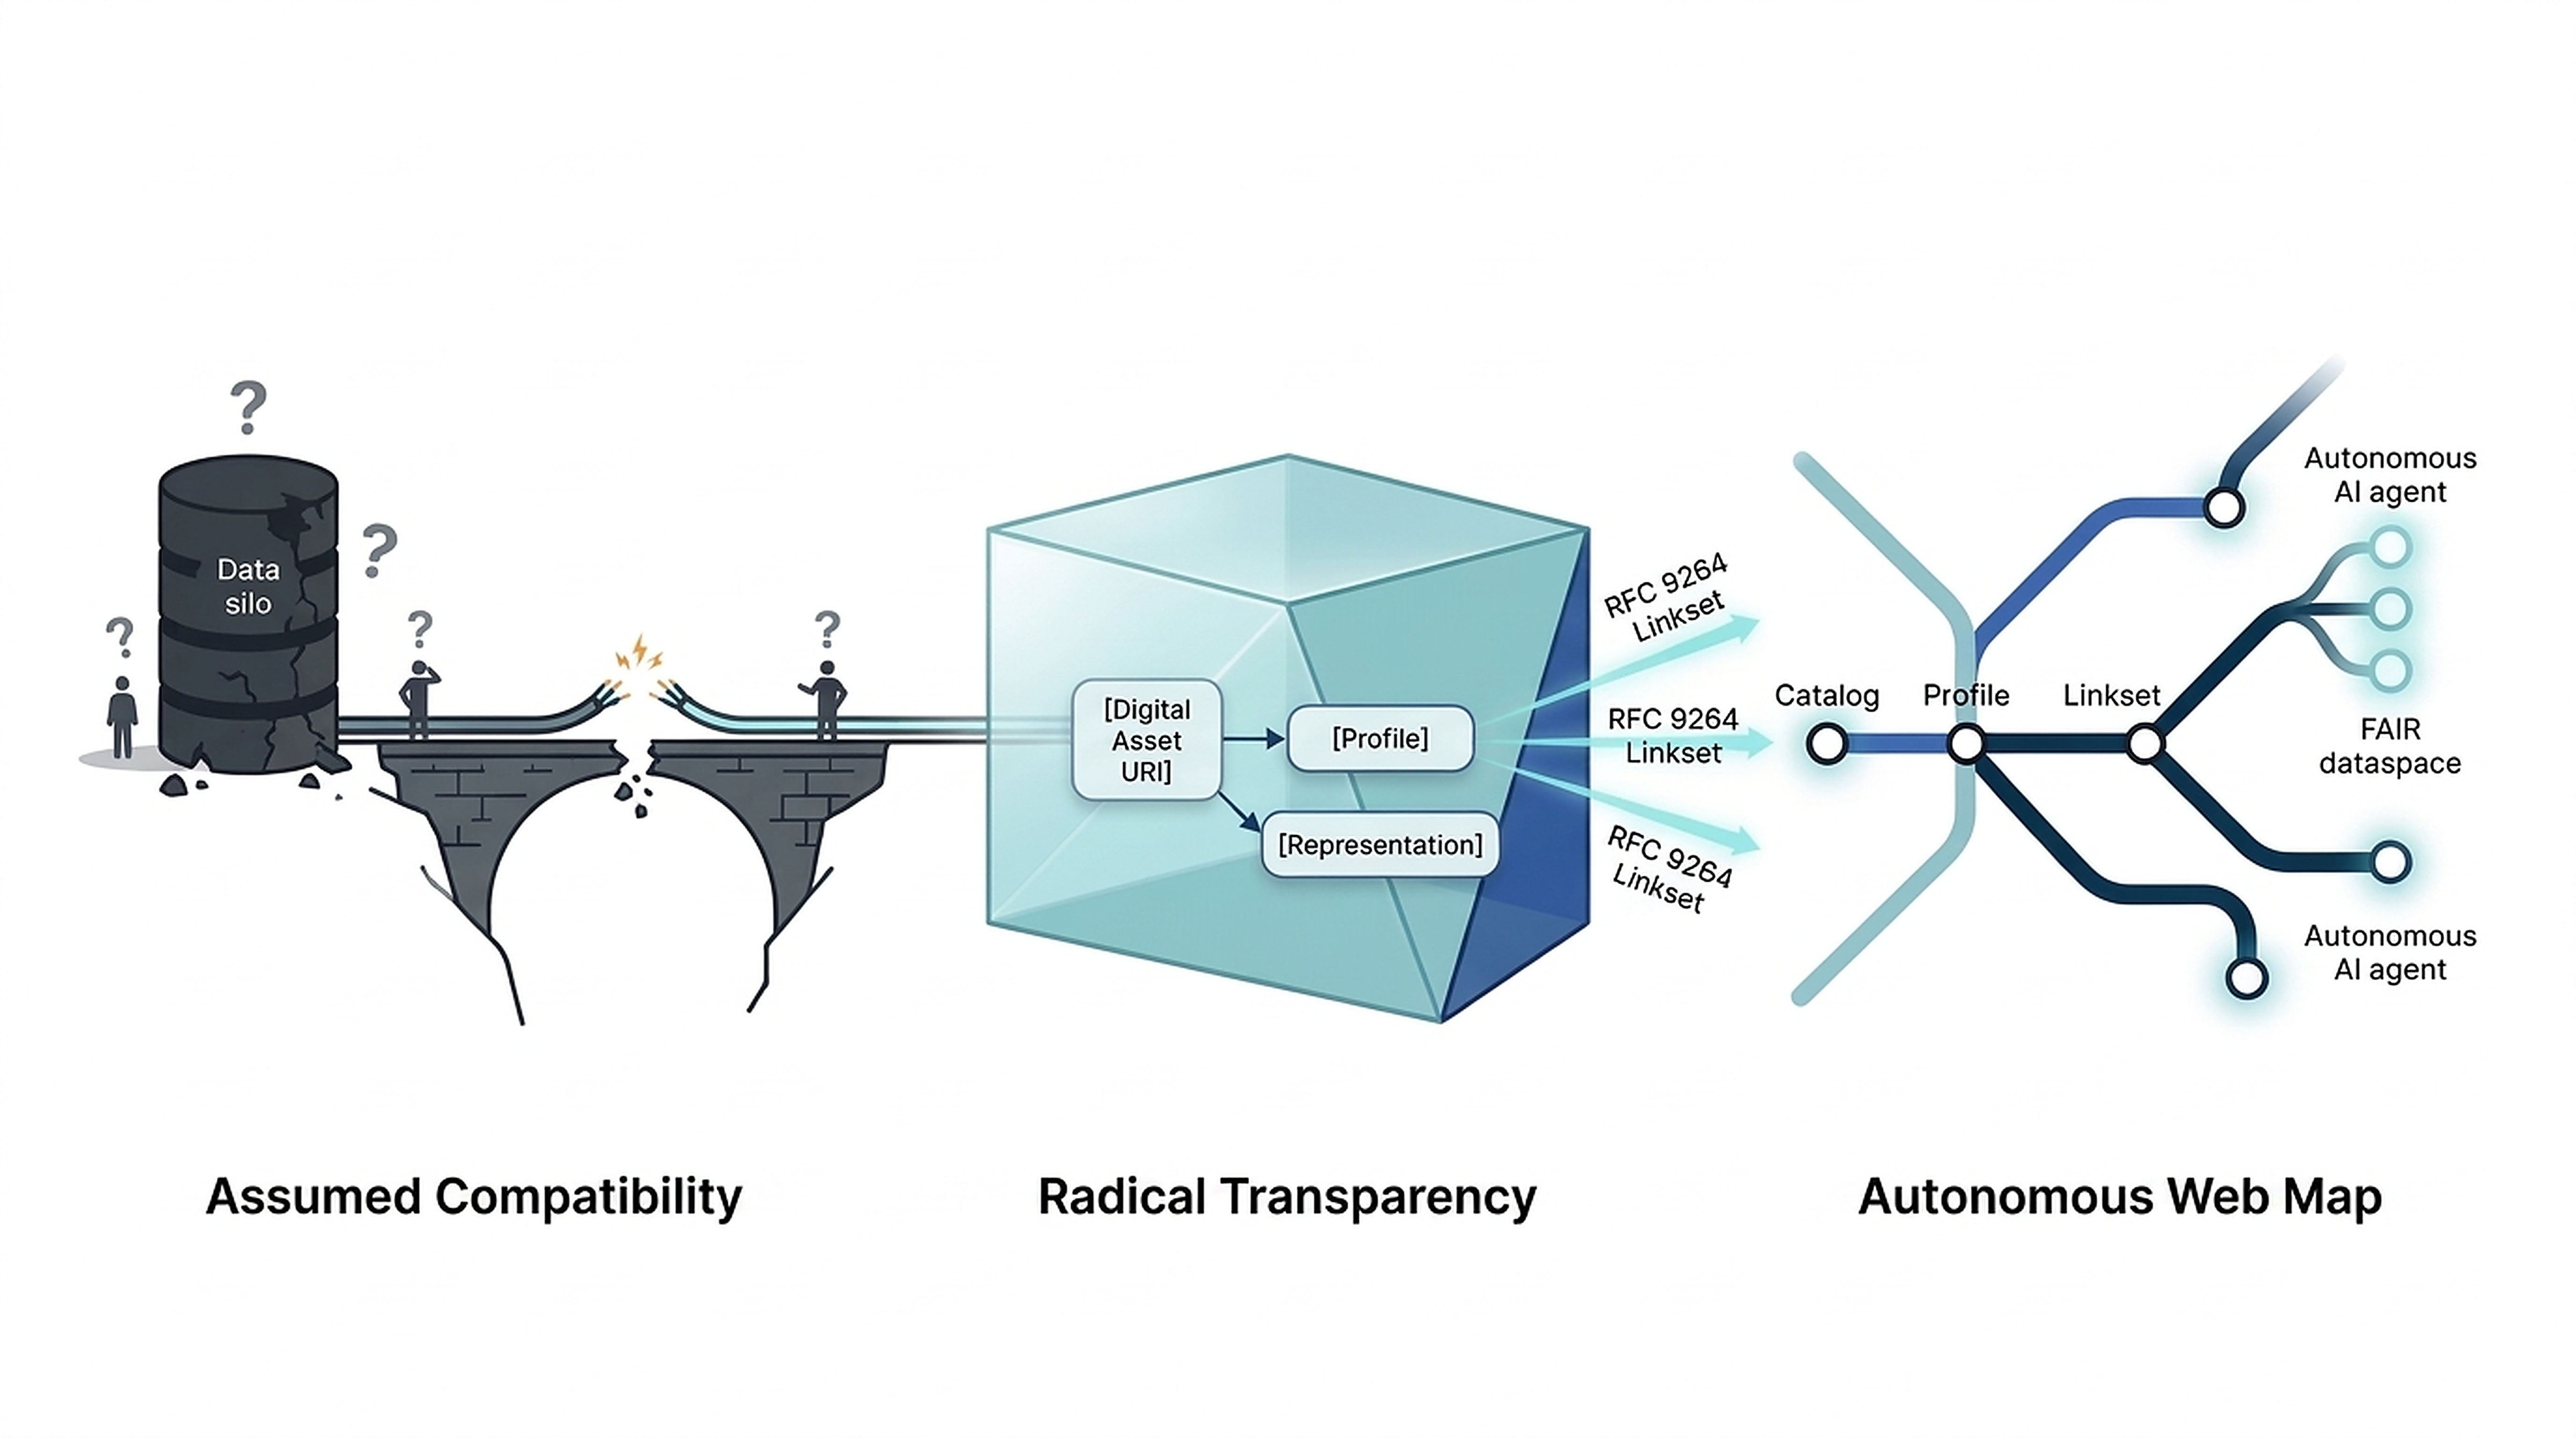
\includegraphics[width=0.96\linewidth]{hero_infographic_hd.png}\\[-0.02cm]
  {\color{vlizSlateMuted}\normalsize \textbf{Figure 1:} \textbf{Radical Transparency} shifts the architectural burden from consumer inference to producer declaration. Moving from fractured data silos and assumed compatibility (\textit{left}), digital assets declare explicit conformity profiles via RFC 9264 linksets (\textit{center}), enabling autonomous AI agents and FAIR dataspaces to navigate web resources like an interconnected transit network (\textit{right}).}
  \vspace{-0.1cm}
}

% ==============================================================================
% 5. BOTTOM 2-COLUMN FLANKING BAND: 4 PILLARS & DUAL QR ACCESS
% ==============================================================================
\begin{columns}
  % ---- Bottom-Left: The 4 Strategic Pillars ----
  \column{0.50}
  \block{3. The 4 Strategic Pillars (2025--2030)}{
    \textbf{Concrete Workplan for Scalable Interoperability:}
    \vspace{0.1cm}

    \noindent
    \begin{minipage}{0.49\linewidth}
      \begin{tcolorbox}[colback=vlizLightTeal,colframe=vlizBanner,arc=4mm,boxrule=1.5pt,left=4mm,right=4mm,top=2.5mm,bottom=2.5mm]
        {\color{vlizNavy}\bfseries 1. Linkset Usage Patterns}\\[2pt]
        {\small 10 documented patterns (RFC 9264/8288) solving Broken Chains \& Semantic Drift.}
      \end{tcolorbox}
    \end{minipage}\hfill
    \begin{minipage}{0.49\linewidth}
      \begin{tcolorbox}[colback=vlizLightTeal,colframe=vlizBanner,arc=4mm,boxrule=1.5pt,left=4mm,right=4mm,top=2.5mm,bottom=2.5mm]
        {\color{vlizNavy}\bfseries 2. Cross-Org Alignment}\\[2pt]
        {\small Shared lightweight bootstrap uniting EOSC-if, CDIF, OGC, RO-Crate, and ODIS.}
      \end{tcolorbox}
    \end{minipage}

    \vspace{0.16cm}
    \noindent
    \begin{minipage}{0.49\linewidth}
      \begin{tcolorbox}[colback=vlizHeroBg,colframe=vlizBorder,arc=4mm,boxrule=1.5pt,left=4mm,right=4mm,top=2.5mm,bottom=2.5mm]
        {\color{vlizNavy}\bfseries 3. Practical Toolchain}\\[2pt]
        {\small Reference tools (\texttt{wrx}, \texttt{stitch}, \texttt{rdf-webcomponents}) for automated discovery.}
      \end{tcolorbox}
    \end{minipage}\hfill
    \begin{minipage}{0.49\linewidth}
      \begin{tcolorbox}[colback=vlizHeroBg,colframe=vlizBorder,arc=4mm,boxrule=1.5pt,left=4mm,right=4mm,top=2.5mm,bottom=2.5mm]
        {\color{vlizNavy}\bfseries 4. Open Profile Market}\\[2pt]
        {\small Federated, DNS-like open profile registers replacing centralized monopolies.}
      \end{tcolorbox}
    \end{minipage}

    \vspace{0.14cm}
    \begin{tcolorbox}[colback=vlizLightTeal,colframe=vlizTeal,arc=4mm,boxrule=1.5pt,left=5mm,right=5mm,top=2.5mm,bottom=2.5mm]
      {\color{vlizNavy}\bfseries Core Separation of Concerns:} {\small Servers provide machine-actionable typed links; clients and autonomous agents handle contextualization, customization, and user interaction.}
    \end{tcolorbox}
    \vspace*{14.3mm}
  }

  % ---- Bottom-Right: London Tube Analogy & Dual QR Codes ----
  \column{0.50}
  \block{4. Web Navigation \& Digital Access}{
    \begin{tcolorbox}[colback=vlizLightTeal,colframe=vlizBanner,arc=4mm,boxrule=1.5pt,left=5mm,right=5mm,top=2.5mm,bottom=2.5mm]
      {\color{vlizNavy}\bfseries The London Tube Navigation Analogy}\\[2pt]
      {\small At any web resource, local linksets map out the direct neighborhood. Typed link relations act as map symbology and color legends, telling autonomous agents exactly where to go next.}
    \end{tcolorbox}

    \vspace{0.14cm}
    \noindent
    \begin{minipage}{0.49\linewidth}
      \begin{tcolorbox}[colback=vlizHeroBg,colframe=vlizNavy,arc=4mm,boxrule=1.5pt,halign=center,top=2.5mm,bottom=2.5mm]
        {\color{vlizNavy}\bfseries Position Paper PDF}\\[4pt]
        
\includegraphics[width=3.6cm,height=3.6cm]{qr_radical_paper.png}\\[4pt]
        {\small \textbf{open-science.vliz.be}}
      \end{tcolorbox}
    \end{minipage}\hfill
    \begin{minipage}{0.49\linewidth}
      \begin{tcolorbox}[colback=vlizHeroBg,colframe=vlizTeal,arc=4mm,boxrule=1.5pt,halign=center,top=2.5mm,bottom=2.5mm]
        {\color{vlizNavy}\bfseries Linkset Patterns}\\[4pt]
        
\includegraphics[width=3.6cm,height=3.6cm]{qr_linkset_patterns.png}\\[4pt]
        {\small \textbf{EOSC-if Proposals}}
      \end{tcolorbox}
    \end{minipage}

    \vspace{0.14cm}
    \begin{tcolorbox}[colback=vlizHeroBg,colframe=vlizBorder,arc=4mm,boxrule=1.5pt,halign=center,top=2.2mm,bottom=2.2mm]
      {\small \textbf{Open Solution Proposals:} \texttt{github.com/eosc-semantic-interop/if-solutions-proposals}}
    \end{tcolorbox}
    \vspace*{2.0mm}
  }
\end{columns}

% ==============================================================================
% 6. FOOTER (References & AI Disclosure)
% ==============================================================================
\block{}{
  \footnotesize
  \begin{minipage}{0.98\linewidth}
    \textbf{References:} [1] Wilde \& Van de Sompel (2022). \textit{Linkset: RFC 9264}. IETF. \quad [2] Nottingham (2017). \textit{Web Linking: RFC 8288}. IETF. \quad [3] Simonis et al. (2026). \textit{Machine-Interpretable Standards Ecosystem: OGC 26-021}. \quad [4] Portier et al. (2026). \textit{Radical Transparency: A Vision for Scalable Interoperability}. VLIZ Open Science Team.\\
    \textbf{AI Disclosure:} Conceptual synthesis assisted by Agentic AI; system vision, architecture, and Linkset patterns by the authors. \quad $\vert$ \quad \textbf{VLIZ Open Science Team 2026}
  \end{minipage}
}

\end{document}
